\section{Desarrollo}

\subsection{Planteo del Sistema}



\begin{wrapfigure}{r}{0.5\textwidth}
  \vspace{-20pt}
  \begin{center}
    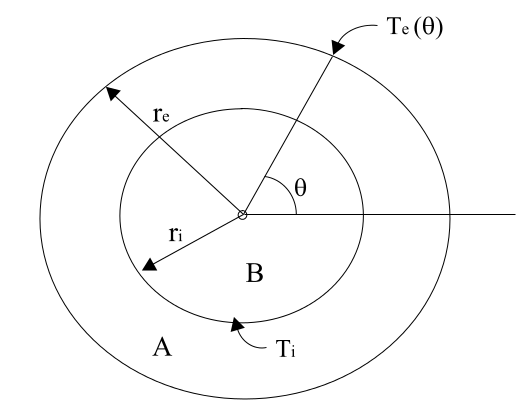
\includegraphics[scale= 0.4]{../Horno.png}
  \end{center}
  \vspace{-20pt}
  \caption{Corte del horno}
  \vspace{-10pt}
  \label{fig:corteHorno}
\end{wrapfigure}


Una instancia del problema equivale a un corte del horno como se ilustra en la figura ~\ref{fig:corteHorno}. Dado que la medición de temperatura en el horno puede realizarse en infinitos puntos, discretizamos el problema fijando la ubicación de los mismos de la siguiente manera; Dividimos el horno en \textbf{\textit{n}} cantidad de ángulos de tamaño $\Delta_{\theta}$ y en \textbf{\textit{m + 1}} cantidad de radios, de tamaño $\Delta_{r}$. Analizaremos las temperaturas en los puntos donde se unen las divisiones entre ángulos y radios. Recordemos que los puntos de la pared interna y externa son dato.\\
\\

La temperatura en un punto $t_{(j,k)}$, con $j \in [0, m]$ y $k \in [0, n)$ estará determinado por la ecuación de Laplace descripta a continuación:


$$ \frac{\partial^{2}T(r,\theta)}{\partial r^{2}} + \frac{1}{r} \frac{\partial T(r,\theta)}{\partial r} + \frac{1}{r^{2}} \frac{\partial^{2}T(r,\theta)}{\partial \theta^{2}} = 0$$\\

Sin embargo utilizaremos una aproximación de esta función que depende de los cuatro puntos que rodean a $t_{(j,k)}$:


$$ \frac{t_{(j-1,k)} - 2t_{(j,k)} + t_{(j+1,k)}}{\Delta_{r} ^{2}} + \frac{1}{r} \frac{t_{(j,k)} - t_{(j-1,k)}}{\Delta_{r}} + \frac{1}{r^{2}} \frac{t_{(j,k-1)} - 2t_{(j,k)} + t_{(j,k+1)}}{\Delta_{\theta} ^{2}} = 0$$

Despejamos las incógnitas $t_{(j,k)}$, $t_{(j+1,k)}$, $t_{(j-1,k)}$, $t_{(j,k+1)}$ y $t_{(j,k-1)}$ para obtener una ecuación (un sistema de ecuaciones) que dependa de ellas. Resulta la siguiente fórmula:



$$  t_{(j,k)} (-\frac{2}{\Delta^2_r}+\frac{1}{r \Delta_r}-\frac{2}{r^2 \Delta^2_\theta}) + t_{(j+1,k)} (\frac{1}{\Delta^2_r}) + t_{(j-1,k)} (\frac{1}{\Delta^2_r}-\frac{1}{r \Delta_r}) + t_{(j,k+1)} (\frac{1}{r^2 \Delta^2_\theta}) + t_{(j,k-1)} (\frac{1}{r^2 \Delta^2_\theta}) = 0$$ \\


Una vez planteadas estas ecuaciones para cada $ t_{(j,k)} $, resolvemos que el sistema $Ax = b$ estará formado por $n*m$ ecuaciones con la misma cantidad de incógnitas. El valor lo justificamos debido a la cantidad de combinaciones entre los índices j y k (cantidad de ángulos por cantidad de radios). Otra forma de razonar este resultado es pensando que en cada anillo generado por la partición del horno en \textbf{\textit{m + 1}} radios, habrá \textbf{\textit{n}} incógnitas generadas a su vez por la particion en ángulos. \\
Esta cantidad incluye los valores $t_{(0,k)}$ y $t_{(n-1,k)}$ (los valores de temperatura en la pared interior y exterior respectivamente), por lo que en sus ecuaciones habrá un único coeficiente con valor 1 en la posición que corresponde a estas incógnitas y su valor b será el que se pase por parámetro. Para el resto de los $t_{(j,k)}$ los coeficientes corresponderan a los coeficientes descriptos en la ecuación de arriba, y su b será cero, también respetando dicha ecuación.

\subsection{Orden de los coeficientes}

Para conseguir una matriz banda, decidimos ordenar los coeficientes de manera creciente respecto al índice \textbf{\textit{j}} para los radios, y luego respecto a \textbf{\textit{k}} el índice de los ángulos. Para ilustrar el orden impuesto, exponemos el siguiente ejemplo



%---------------------------------------------------------------------

\subsection{Análisis de Coeficientes}
A partir de las aproximaciones de las derivadas parciales de la función $T$ distribuimos los términos para conocer los coeficientes asociados a cada punto del cual depende el valor de la temperatura que queremos conocer para un $j,k$ dado. Se debe cumplir la siguiente ecuación: \\
$$t_{(j-1, k)} (\frac{1}{\Delta^2_r}-\frac{1}{r \Delta_r}) +
t_{(j, k)} (-\frac{2}{\Delta^2_r}+\frac{1}{r \Delta_r}-\frac{2}{r^2 \Delta^2_\theta}) + 
t_{(j+1, k)} (\frac{1}{\Delta^2_r}) + 
t_{(j, k-1)} (\frac{1}{r^2 \Delta^2_\theta}) +
t_{(j, k+1)} (\frac{1}{r^2 \Delta^2_\theta}) = 0 $$ \\

Analizamos los casos en que los coeficientes obtenidos a partir de la discretización de las derivadas parciales asociados a cada punto se anulan, es decir, para que $r, \Delta_r,$ y $\Delta_\theta$ el coeficiente se anula. \\
Para el coeficiente asociado a $t_{(j-1, k)}$, $r$ debe valer $\Delta_r$. Como $r_j = (j \Delta_r) + r_i$ esto se cumple si $j$ vale 1 y $r_i$ vale cero, o $j$ vale cero y $r_i$ vale $\Delta_r$. Para el primer caso, significa que el horno no tiene radio interno, mientras que la segunda no puede suceder puesto que la ecuación la cumplen solo las temperaturas entre el radio interno y el externo (no incluidos) y si $j$ vale cero, indica que es el radio interno.
Para los coeficientes de $t_{(j+1, k)}$, $t_{(j, k-1)}$ y $t_{(j, k+1)}$, los coeficientes nunca se anulan. \\
Por último, para el coeficiente asociado a $t_{(j, k)}$, desarrollamos las sumas e igualamos a cero. \\
$$\frac{-2r^2 \Delta^2_\theta + r \Delta_r \Delta^2_\theta - 2 \Delta^2_r}{\Delta^2_r r^2 \Delta^2_\theta} = 0$$\\
El término inferior nunca se anula, por lo que debería anularse el término superior. Observamos que corresponde a una función cuadrática siendo $r$ la variable. Desarrollamos la fórmula de Bhaskara obteniendo: \\
$$r = \frac{\Delta_r}{4} \pm \frac{\sqrt{\Delta^2_r \Delta^4_\theta - 16 \Delta_\theta \Delta^2_r}}{4 \Delta^2_\theta}$$ \\
El análisis se vuelve muy complicado, pero nos valemos de saber que para que el planteo tenga sentido, $r$ debe ser mayor o igual que $\Delta_r$.
El segundo miembro es siempre positivo, por lo que si se le resta algo positivo a $\frac{\Delta_r}{4}$, seria aún menor, por lo tanto solo queda analizar el caso en que se suman los términos. Para que se cumpla la condición $\Delta_r \leq r$, queremos encontrar los $\Delta_r$ y $\Delta_\theta$ tal que: \\
$$\frac{3 \Delta_r}{4}  \leq \frac{\sqrt{\Delta^2_r \Delta^4_\theta - 16 \Delta_\theta \Delta^2_r}}{d \Delta^2_\theta} $$ \\
Para este fin, utilizamos la página web $www.wolframalpha.com$ para encontrar las soluciones al problema, las cuales indican que si $\Delta_r$ es positivo, $\Delta_\theta$ debe ser menor a cero y viceversa. Por lo tanto, el coeficiente se anula solamente para valores que no tienen sentido dentro del problema. \\
%http://www.wolframalpha.com/input/?i=sqrt%28x^2+y^4+-+16+x^2+y%29+%2F+%284*y^2%29+%3E%3D+3x%2F4
Con este análisis, concluimos que los coeficientes obtenidos de la ecuación no se anulan en los casos en que el problema planteado tiene sentido.

%---------------------------------------------------------------------

\subsection{Análisis de Pivoteo}

Para justificar que en la matriz banda no se produce pivoteo al aplicarse el algoritmo de Eliminación Gaussiana, procedemos a demostrar que la matriz banda es diagonal dominante. Con esto llegamos a la conclusión de que es no singular y luego....
%TODO: no se como sigue el hilo, claramente falta terminarlo. Se que si demostramos que tiene factorizacin LU entonces por una propiedad vista en clase, las submatrices ppales son no singulares (inversibles), por lo tanto podriamos aplicar el teorema ese raro que encontro axel del que no tenemos nada. Pero si no lo usamos que haciamos??

%---------------------------------------------------------------------


\subsubsection{A es diagonal dominante}
Queremos ver que A es diagonal dominante, es decir, que se cumple la siguiente inecuación:\\
$$\mid \frac{1}{\Delta^2_r}-\frac{1}{r \Delta_r}\mid +
\mid \frac{1}{\Delta^2_r} \mid + 
\mid \frac{1}{r^2 \Delta^2_\theta} \mid +
\mid \frac{1}{r^2 \Delta^2_\theta} \mid
\leq \mid -\frac{2}{\Delta^2_r}+\frac{1}{r \Delta_r}-\frac{2}{r^2 \Delta^2_\theta} \mid$$  \\
Primero, nos deshacemos de los módulos. El primer término es negativo solo cuando $r < {\Delta_r}$, pero esto no sucede debido a que $r= j \Delta_r + r_i$, con $j$ natural y $r_i$ real positivo. El resto de los términos a la izquierda de la desigualdad tambien son positivos debido a que todas las viariables estan elevadas al cuadrado, por lo tanto es equivalente no tomar módulo para estos términos. \\
Para el término de la derecha, $-\frac{2}{r^2 \Delta^2_\theta}$ siempre es negativo, por lo que para que el término sea positivo, $-\frac{2}{\Delta^2_r}+\frac{1}{r \Delta_r}$ debe de ser necesariamente positivo. Sin embargo, esto solo puede ocurrir cuando $r < \frac{\Delta_r}{2}$, por lo que siempre resulta negativo por el argumento anterior. De este modo, si multiplicamos este término por -1, obtenemos un número positivo. La inecuación resultante es: \\ 
$$ \frac{1}{\Delta^2_r}-\frac{1}{r \Delta_r} +  
\frac{1}{\Delta^2_r} + 
\frac{1}{r^2 \Delta^2_\theta} +
\frac{1}{r^2 \Delta^2_\theta}
\leq \frac{2}{\Delta^2_r}-\frac{1}{r \Delta_r}+\frac{2}{r^2 \Delta^2_\theta}$$ \\

Sumamos los términos y obtenemos: \\
$$\frac{2}{\Delta^2_r}-\frac{1}{r \Delta_r}+\frac{2}{r^2 \Delta^2_\theta} \leq \frac{2}{\Delta^2_r}-\frac{1}{r \Delta_r}+\frac{2}{r^2 \Delta^2_\theta}$$ \\
Podemos observar que se cumple la inecuación como queríamos demostrar, y en particular, vale la igualdad.


%---------------------------------------------------------------------

\subsubsection{A es no singular}
Dada la matriz A diagonal dominante, veamos que A es no singular.
Por absurdo supongamos que es singular, esto es, $\exists x\neq 0$ tal que $x \in Nu(A)$.
Como el vector es distinto a cero, existe una coordenada que es mayor al resto. Llamémosla $x_{k}$.


Del sistema de ecuaciones Ax, tomemos la ecuación k, que tiene esta forma:                  

$$ a_{(k, 1)} * x_{1} + a_{(k, 2)} * x_{2} +... + a_{(k, n)} * x_{n} = 0 $$\\

Luego despejamos el término k y aplicamos módulo:\\

 $$ \mid a_{(k, k)} * x_{k} \mid  =  \left \arrowvert - \sum_{j=1,j\neq k}^{n}  a_{(k,j)} * x_{j} \right \arrowvert $$

 $$ \mid a_{(k, k)}\mid * \mid x_{k} \mid \leq \sum_{j=1,j\neq k}^{n} \mid a_{(k,j)}\mid * \mid x_{j} \mid $$


 $$ \mid a_{(k, k)}\mid  = \sum_{j=1,j\neq k}^{n} \mid a_{(k,j)}\mid *  \frac{\mid x_{j} \mid}{\mid x_{k} \mid}$$\\

Anteriormente probamos que A es diagonal dominante y que en particular vale la igualdad. Como cada elemento de la sumatoria (que vale exactamente $a_{(k, k)}$) es multiplicado por $\frac{\mid x_{j} \mid}{\mid x_{k} \mid}$ $\leq 1$, disminuyen su valor, con lo que la sumatoria se reduce y resulta:\\

$$\mid a_{(k,k)} \mid < \sum_{j=1, j\neq k}^{n}\mid a_{(k,j)} \mid $$\\

Lo que es absurdo, pues A era diagonal dominante. El absurdo provino de suponer que A es singular. Luego vale que A es no singular.




%---------------------------------------------------------------------

\subsection{Problemas que nos encontramos durante el desarrollo}

\begin{itemize}
\item Nos encontramos con problemas a la hora de cargar la matriz A de coeficientes. Lo solucionamos realizando ejemplos de un tamaño razonable en papel, y chequeando a mano que las distintas filas estuvieran bien cargadas.

\item Problemas de precisión numérica. Inicialmente los resultados de los\ tests diferían con los resultados de la cátedra. Debido a los problemas inherentes a la aritmética de punto flotante, comenzamos experimentando con distintas maneras de realizar la sumatoria (ordenando los números de mayor a menor y de menor a mayor), ya que pensabamos que estabamos arrastrando un error. Descubrimos que las distintas maneras de realizar las sumatorias diferían en menos de $0,00001$, por lo que concluímos que no estabamos arrastrando errores en las cuentas. Finalmente descubrimos que el error estaba en que la variable $m$ en realidad era $m+1$, y no teníamos eso en cuenta a la hora de calcular $\Delta r$.

\end{itemize}